\chapter{Dasar Teori}
\label{chap:dasar teori}

Pada bab ini dibahas dasar-dasar teori yang diperlukan dalam proses penulisan penelitian mengenai perlindungan \textit{password} dengan entropi personal. Terdapat beberapa hal yang dibahas pada bab ini, yaitu mengenai kriptografi, \textit{Data Encryption Standard}, \textit{Secure Hash Algorithm 512}, otentikasi, eliminasi Gauss-Jordan, \textit{secret sharing}, probabilitas, dan entropi.

\section{Kriptografi}

Pada bagian ini dijelaskan mengenai kriptografi dimulai dari sejarah kriptografi, dan pengertian kriptografi.

\subsection{Sejarah Kriptografi}

Kriptografi berasal dari bahasa Yunani, terdiri dari dua suku kata yaitu, \textit{kripto} dan \textit{graphia}, \textit{kripto} berarti rahasia dan \textit{graphia} berarti tulisan. Jadi, kriptografi berarti teknik atau metode untuk merahasiakan tulisan.

Kemunculan kriptografi ini diawali karena kebutuhan manusia untuk merahasiakan informasi berupa pesan atau tulisan. Pada zaman dahulu kala, kriptografi digunakan untuk merahasiakan tulisan-tulisan mengenai pesan rahasia, strategi perang, dan masih banyak lagi. Salah satu bentuk penggunaan kriptografi pada zaman dahulu kala adalah alat yang dinamakan \textit{scytale}. \textit{Scytale} digunakan oleh tentara Sparta di Yunani untuk mengirimkan pesan rahasia\cite{munir2010matematikadiskrit}.

\subsection{Pengertian Kriptografi}

Zaman sekarang ini, kerahasiaan informasi menjadi hal yang penting. Informasi yang berharga perlu dirahasiakan sehingga tidak diketahui oleh orang yang tidak berhak. Kriptografi berperan dalam merahasiakan informasi berharga tersebut. Jadi, kriptografi adalah ilmu atau seni untuk menjaga kerahasiaan informasi.

Kriptografi memiliki 4 layanan utama\cite{forouzan2007cryptography}:
\begin{enumerate}
	\item Kerahasiaan (\textit{confidentiality})\\
	Layanan ini menjamin bahwa informasi yang dikirimkan tidak diketahui oleh pihak yang tidak berhak melihat atau membacanya.
	\item Integritas (\textit{integrity})\\
	Layanan ini menjamin keaslian dari informasi yang dikirimkan dan menjamin bahwa informasi yang dikirimkan tidak diubah tanpa seijin pengirim informasi.
	\item Otentikasi (\textit{authentication})\\
	Layanan ini menjamin keaslian identitas dari pengirim dan penerima informasi.
	\item Non-repudiasi (\textit{nonrepudiation})\\
	Layanan ini menjamin pengirim dan penerima informasi tidak dapat menyangkal aktivitas yang sudah dilakukan.
\end{enumerate}

\section{Kerahasiaan (\textit{Confidentiality})}

Kerahasian adalah layanan yang menjamin bahwa informasi yang dikirimkan tidak dapat dibaca oleh orang atau pihak yang tidak berhak. Dalam kriptografi, informasi yang bisa dibaca dan dimengerti disebut \textit{plaintext}. Informasi yang sudah dirahasiakan sehingga tidak bisa dibaca dan dimengerti disebut \textit{ciphertext}. Untuk merahasiakan \textit{plaintext}, maka \textit{plaintext} harus diubah menjadi \textit{ciphertext}. Kemudian, untuk bisa membaca kembali informasi yang sudah dirahasiakan, \textit{ciphertext} harus diubah kembali menjadi \textit{plaintext}.

Proses untuk mengubah \textit{plaintext} menjadi \textit{ciphertext} dinamakan enkripsi. Sebaliknya, proses untuk mengubah \textit{ciphertext} menjadi \textit{plaintext} dinamakan dekripsi. Proses enkripsi dan dekripsi ini menggunakan kunci. Kunci adalah sekumpulan huruf, angka, atau simbol. Kunci sifatnya rahasia dan hanya boleh diketahui oleh pemilik informasi.

Dalam proses enkripsi, \textit{plaintext} dipetakan dengan fungsi enkripsi \begin{math}E\end{math} menjadi \textit{ciphertext} menggunakan kunci \begin{math}k\end{math}, seperti pada persamaan \ref{eq:enkripsi}.

\begin{equation}
	E_k(plaintext) = ciphertext
	\label{eq:enkripsi}
\end{equation}

Sementara itu, dalam proses dekripsi, \textit{ciphertext} dipetakan dengan fungsi dekripsi \begin{math}D\end{math} menjadi \textit{plaintext} menggunakan kunci \begin{math}k\end{math} seperti pada persamaan \ref{eq:dekripsi}.

\begin{equation}
	D_k(ciphertext) = plaintext
	\label{eq:dekripsi}
\end{equation}

Proses enkripsi dan dekripsi ini menggunakan sekumpulan fungsi matematika untuk mengubah \textit{plaintext} menjadi \textit{ciphertext} dan sebaliknya. Sekumpulan fungsi matematika yang digunakan dalam proses enkripsi dan dekripsi dinamakan algoritma kriptografi. Menurut penggunaan kuncinya algoritma kriptografi dibagi menjadi 2 jenis, yaitu algoritma kriptografi kunci simetris dan algoritma kriptografi kunci asimetris.

Algoritma kunci simetris menggunakan kunci yang sama untuk proses enkripsi dan dekripsi. Pemilik informasi melakukan proses enkripsi dan dekripsi dengan kunci yang sama sehingga kunci harus dirahasiakan. Contoh dari algoritma kriptografi kunci simetris antara lain, \textit{Data Encryption Standard} (DES), \textit{Advanced Encryption Standard} (AES), \textit{Twofish}, dan \textit{Blowfish}.

Algoritma kunci asimetris menggunakan kunci yang berbeda untuk proses enkripsi dan dekripsi. Pemilik informasi melakukan proses enkripsi menggunakan kunci yang dinamakan kunci publik dan melakukan proses dekripsi menggunakan kunci yang dinamakan kunci pribadi. Kunci publik sifatnya tidak rahasia dan kunci pribadi sifatnya rahasia. Contoh dari algoritma kriptografi kunci asimetris antara lain, Rivest-Shamir-Adleman (RSA), ElGamal, Diffie-Helman, \textit{Digital Signature Algorithm}, dan \textit{Elliptic Curve Digital Signature Algorithm} (ECDSA).

\section{\textit{Data Encryption Standard} (DES)}\label{sec:des}

Pada bagian ini dijelaskan hal-hal mengenai \textit{data encryption standard} dimulai dari sejarah \textit{data encryption standard}, struktur \textit{data encryption standard}, dan proses enkripsi \textit{data encryption standard}.

\subsection{Sejarah}

\textit{Data encryption standard} atau disingkat DES adalah algoritma kriptografi kunci simetris. DES pertama kali dipublikasikan oleh \textit{National Institute of Standards and Technology} (NIST) pada tahun 1973. DES merupakan algoritma enkripsi pertama yang disetujui oleh pemerintah Amerika Serikat untuk digunakan secara luas. Pada bulan Maret 1975, NIST memublikasikan DES sebagai standar enkripsi untuk data pemerintahan atau \textit{Federal Information Processing Standard} (FIPS).

\subsection{Struktur DES}

Masukkan dari DES berupa 64-\textit{bit} \textit{plaintext}. Keluaran dari DES berupa 64-\textit{bit} \textit{ciphertext}. DES menggunakan kunci yang sama pada proses enkripsi dan dekripsi. Panjang kunci dari DES adalah 64-\textit{bit}. Proses enkripsi terdiri dari permutasi awal, putaran dan permutasi akhir. Gambar \ref{fig:prosesenkripsi} menunjukkan proses enkripsi dari DES. Pada bagian selanjutnya dijelaskan mengenai setiap bagian dari proses enkripsi.

\begin{figure}[H]
	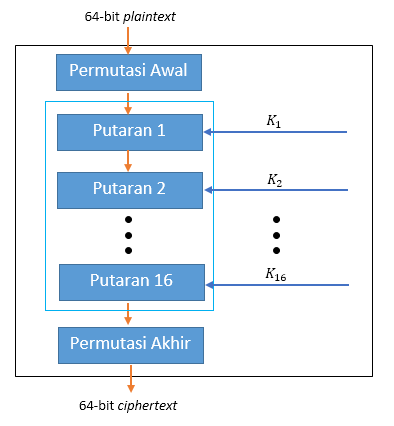
\includegraphics[scale=0.8]{Gambar/proses_enkripsi_des}
	\centering
	\caption{Proses Enkripsi}\label{fig:prosesenkripsi}
\end{figure}

\subsection{Permutasi Awal}\label{subsec:permutasiawal}

Permutasi awal dalam DES menggunakan matriks permutasi \begin{math}mp\end{math}. Masukan dari matriks permutasi \begin{math}mp\end{math} adalah \textit{plaintext}. Tabel \ref{table:awal} menunjukkan matriks permutasi \begin{math}mp\end{math}.

\begin{table}[H]
	\centering
	\caption{Matriks Permutasi Awal}\label{table:awal}
	\begin{tabular}{|l|l|l|l|l|l|l|l|}
			\hline
			58	&	50	&	42	&	34	&	26	&	18	&	10	&	2	\\ \hline
			60	&	52	&	44	&	36	&	28	&	20	&	12	&	4	\\ \hline
			62	&	54	&	46	&	38	&	30	&	22	&	14	&	6	\\ \hline
			64	&	56	&	48	&	40	&	32	&	24	&	16	&	8	\\ \hline
			57	&	49	&	41	&	33	&	25	&	17	&	9	&	1	\\ \hline
			59	&	51	&	43	&	35	&	27	&	19	&	11	&	3	\\ \hline
			61	&	53	&	45	&	37	&	29	&	21	&	13	&	5	\\ \hline
			63	&	55	&	47	&	39	&	31	&	23	&	15	&	7	\\ \hline
	\end{tabular}
\end{table}

Cara kerja dari proses permutasi adalah sebagai berikut. Angka yang ditunjukkan pada posisi ke-\begin{math}i\end{math} matriks \begin{math}mp\end{math} merupakan posisi \textit{bit} dari masukan, sedangkan \begin{math}i\end{math} menunjukkan posisi \textit{bit} dari keluaran. Proses permutasi ditunjukkan oleh persamaan \ref{eq:permutasi}.

\begin{equation}
	keluaran_i = masukan_{p_i}
	\label{eq:permutasi}
\end{equation}

Sebagai contoh, posisi ke-1 dari matriks \begin{math}mp\end{math} menunjukkan angka 58. Maka, \textit{bit} ke-58 dari masukan akan menjadi \textit{bit} ke-1 dari keluaran. Contoh lainnya, posisi ke-62 dari matriks $mp$ menunjukkan angka 23. Maka, \textit{bit} ke-23 dari masukan akan menjadi \textit{bit} ke-62 dari keluaran.

\subsection{Pembangunan Kunci Putaran}

DES menggunakan kunci dengan panjang 64-\textit{bit}. Kunci ini perlu diubah menjadi kunci untuk setiap putaran DES dengan panjang masing-masing 48-\textit{bit}. Proses pembangunan kunci putaran terdiri dari \textit{parity drop}, \textit{shift left}, dan permutasi \textit{P-box}. Gambar \ref{fig:keygenerate} menunjukkan keseluruhan proses dari pembangunan kunci putaran. Pada bagian ini akan dijelaskan masing-masing proses dari pembangunan kunci putaran.

%diagram
\begin{figure}[H]
	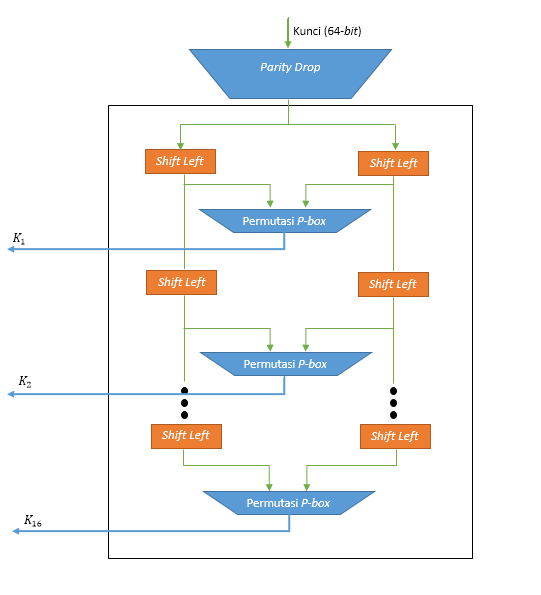
\includegraphics[scale=0.7]{Gambar/key_generate}
	\centering
	\caption{Proses Pembangunan Kunci Putaran}\label{fig:keygenerate}
\end{figure}

\subsubsection{\textit{Parity Drop}}

Pada proses ini, \textit{parity bit} akan dihilangkan dari kunci masukan. \textit{Bit} yang dihilangkan adalah \textit{bit} posisi kelipatan 8, yaitu posisi ke-8, posisi ke-16, posisi ke-24, dan seterusnya sampai posisi ke-64. Proses penghilangan \textit{parity bit} ini menggunakan matriks permutasi \begin{math}p\end{math} seperti ditunjukkan pada Tabel \ref{table:parity_drop}. Cara kerja proses permutasi sama dengan cara kerja proses permutasi pada tahap permutasi awal (Subbab \ref{subsec:permutasiawal}).

\begin{table}[H]
	\begin{center}
		\caption{Matriks Permutasi untuk \textit{Parity Drop}}\label{table:parity_drop}
		\begin{tabular}{|l|l|l|l|l|l|l|l|}
				\hline
				57	&	49	&	41	&	33	&	25	&	17	&	9		&	1		\\ \hline
				58	&	50	&	42	&	34	&	26	&	18	&	10	&	2		\\ \hline
				59	&	51	&	43	&	35	&	27	&	19	&	11	&	3		\\ \hline
				60	&	52	&	44	&	36	&	63	&	55	&	47	&	39	\\ \hline
				31	&	23	&	15	&	7		&	62	&	54	&	46	&	38	\\ \hline
				30	&	22	&	14	&	6		&	61	&	53	&	45	&	37	\\ \hline
				29	&	21	&	13	&	5		&	28	&	20	&	12	&	4		\\ \hline
		\end{tabular}
	\end{center}
\end{table}

Hasil akhir dari proses ini kunci dengan panjang 56-bit.

\subsubsection{\textit{Shift Left}}

Pada proses ini, kunci hasil proses \textit{parity drop} dibagi menjadi 2 bagian dengan panjang masing-masing 28-\textit{bit}, yaitu bagian kiri (\textit{L}) dan bagian kanan (\textit{R}). \begin{math}L\end{math} dan \begin{math}R\end{math} akan digeser ke arah kiri secara sirkular sebanyak 1 atau 2 \textit{bit} tergantung dari urutan putaran. Ketentuan banyak \textit{bit} yang digeser adalah sebagai berikut.

\begin{itemize}
	\item Untuk putaran ke-1, 2, 9, dan 16 maka \begin{math}L\end{math} dan \begin{math}R\end{math} akan digeser ke arah kiri secara sirkular sebanyak 1 \textit{bit}.
	\item Untuk putaran ke-3, 4, 5, 6, 7, 8, 10, 11, 12, 13, 14, dan 15, \begin{math}L\end{math} dan \begin{math}R\end{math} akan digeser ke arah kiri secara sirkular sebanyak 2 \textit{bit}.
\end{itemize}

Sebagai contoh, misalkan \begin{math}L\end{math} dan \begin{math}R\end{math} pada persamaan \ref{eq:L} dan \ref{eq:R}.

\begin{equation}
	L = 1001\: 1010\: 1000\: 0110\: 0110\: 1111\: 1101
	\label{eq:L}
\end{equation}

\begin{equation}
	R = 0001\: 0100\: 0111\: 1110\: 1010\: 0101\: 1011
	\label{eq:R}
\end{equation}

Untuk putaran ke-1, 2, 9, dan 16 maka hasil dari \begin{math}L\end{math} dan \begin{math}R\end{math} akan seperti yang ditunjukkan pada persamaan \ref{eq:L1} dan \ref{eq:R1}.

\begin{equation}
	L = 0011\: 0101\: 0000\: 1100\: 1101\: 1111\: 1011
	\label{eq:L1}
\end{equation}

\begin{equation}
	R = 0010\: 1000\: 1111\: 1101\: 0100\: 1011\: 0110
	\label{eq:R1}
\end{equation}

Sementara itu, jika untuk putaran ke-3, 4, 5, 6, 7, 8, 10, 11, 12, 13, 14, dan 15 akan seperti yang ditunjukkan pada persamaan \ref{eq:L2} dan \ref{eq:R2}.

\begin{equation}
	L = 0110\: 1010\: 0001\: 1001\: 1011\: 1111\: 0110
	\label{eq:L2}
\end{equation}

\begin{equation}
	R = 0101\: 0001\: 1111\: 1010\: 1001\: 0110\: 1100
	\label{eq:R2}
\end{equation}

Kemudian, \begin{math}L\end{math} dan \begin{math}R\end{math} akan disatukan kembali sehingga panjangnya menjadi 56-\textit{bit}.

\subsubsection{Permutasi \textit{P-box}}

Tahap ini adalah proses permutasi untuk mengubah kunci dari proses \textit{Shift Left} dengan panjang 56-\textit{bit} menjadi kunci putaran dengan panjang 48-\textit{bit}. Tabel \ref{table:kompresi_p} menunjukkan matriks permutasi\textit{ P-box} yang digunakan untuk proses ini.

\begin{table}[H]
	\begin{center}
		\caption{Matriks kompresi \textit{P-box}}\label{table:kompresi_p}
		\begin{tabular}{|l|l|l|l|l|l|l|l|}
				\hline
				14	&	17	&	11	&	24	&	1	&	5	&	3	&	28	\\ \hline
				15	&	6	&	21	&	10	&	23	&	19	&	12	&	4	\\ \hline
				26	&	8	&	16	&	7	&	27	&	20	&	13	&	2	\\ \hline
				41	&	52	&	31	&	37	&	47	&	55	&	30	&	40	\\ \hline
				51	&	45	&	33	&	48	&	44	&	49	&	39	&	56	\\ \hline
				32	&	29	&	36	&	50	&	42	&	46	&	53	&	34	\\ \hline
		\end{tabular}
	\end{center}
\end{table}

Hasil keluaran dari proses ini adalah kunci putaran dengan panjang 48-\textit{bit} dan siap dipakai untuk masing-masing putaran.

\subsection{Putaran}

DES terdiri dari 16 putaran. Setiap putaran adalah jaringan Feistel yang akan dijelaskan pada bagian selanjutnya. Gambar \ref{fig:putarandes} menunjukkan ilustrasi dari 16 putaran dari DES.

\begin{figure}[H]
	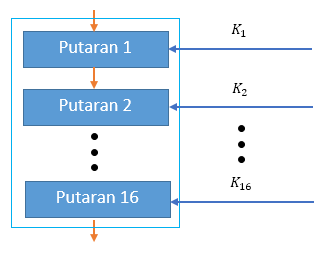
\includegraphics[scale=0.8]{Gambar/putaran_des}
	\centering
	\caption{Putaran dalam DES}\label{fig:putarandes}
\end{figure}

\subsubsection{Jaringan Feistel}

Pada bagian ini akan dijelaskan mengenai sejarah singkat dari jaringan Feistel dan pembahasan jaringan Fesitel.

\subsubsection{Sejarah Singkat}

Jaringan Feistel diciptakan oleh ilmuwan asal Jerman bernama Horst Feistel. Horst Feistel mempublikasikan jaringan ini pada tahun 1973. Jaringan Feistel banyak digunakan dalam berbagai skema enkripsi khususnya digunakan dalam DES.

\subsubsection{Pembahasan}

Masukan dari jaringan Feistel adalah \textit{plaintext} dengan panjang 64-\textit{bit} dan keluaran dari jaringan Feistel adalah \textit{ciphertext} dengan panjang 64-\textit{bit}. Jaringan Feistel menggunakan kunci \begin{math}K\end{math} dan fungsi enkripsi \begin{math}f\end{math} dalam pemrosesan \textit{plaintext}. Selanjutnya akan dijelaskan langkah-langkah pemrosesan \textit{plaintext} pada jaringan Feistel.

\begin{enumerate}
	\item \textit{Plaintext} dibagi menjadi 2 bagian sama panjang, yaitu bagian kiri (\begin{math}L_{i-1}\end{math}) dan bagian kanan (\begin{math}R_{i-1}\end{math}). Huruf \begin{math}i\end{math} menunjukkan urutan dari putaran. Panjang masing-masing bagian adalah 32-\textit{bit}.
	\item Bagian kanan (\begin{math}R_{i-1}\end{math}) pada \textit{plaintext} akan menjadi bagian kiri (\begin{math}L_i\end{math}) dari \textit{ciphertext}. Persamaan \ref{eq:swap} menunjukkan langkah yang sudah dijelaskan.
	\begin{equation}
		L_i = R_{i-1}
		\label{eq:swap}
	\end{equation}
	\item Untuk memperoleh bagian kanan dari \textit{ciphertext} (\begin{math}R_i\end{math}), bagian kanan dari \textit{plaintext} (\begin{math}R_{i-1}\end{math}) dan kunci putaran \begin{math}K_i\end{math} dipetakan dengan fungsi \begin{math}f\end{math}. Kemudian, hasil pemetaan dengan fungsi \begin{math}f\end{math} akan di \textit{exclusive-or} (XOR) dengan bagian kiri dari plaintext (\begin{math}L_{i-1}\end{math}). Persamaan \ref{eq:xor} menunjukkan langkah yang sudah dijelaskan.
	\begin{equation}
		R_i = L_{i-1} \oplus f(R_{i-1}, K_i)
		\label{eq:xor}
	\end{equation}
	\item Hasil akhirnya berupa \textit{ciphertext} dengan 2 bagian sama panjang, yaitu bagian kiri (\begin{math}L_i\end{math}) dan bagian kanan (\begin{math}R_i\end{math}). 
\end{enumerate}

Gambar \ref{fig:jaringanfeistel} menunjukkan ilustrasi dari langkah-langkah yang sudah dijelaskan.

%diagram
\begin{figure}[H]
	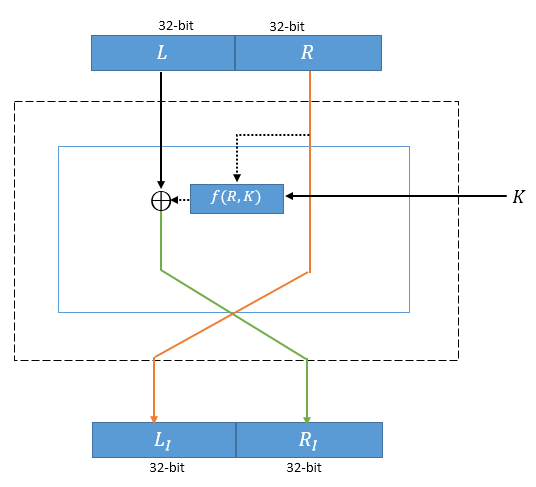
\includegraphics[scale=0.6]{Gambar/jaringan_feistel}
	\centering
	\caption{Jaringan Feistel}\label{fig:jaringanfeistel}
\end{figure}

\subsubsection{Fungsi DES}

Fungsi DES adalah fungsi \begin{math}f\end{math} yang digunakan dalam jaringan Feistel pada Gambar \ref{fig:jaringanfeistel}. Fungsi DES terdiri dari 4 bagian, yaitu ekspansi \textit{P-box}, operasi XOR, substitusi \textit{S-box}, dan permutasi. Pada bagian selanjutnya akan dijelaskan masing-masing bagian dari fungsi DES.

\subsubsection{Ekspansi \textit{P-box}}

Pada bagian ini, masukan berupa blok bagian kanan dari \textit{plaintext} (\begin{math}R\end{math}) dengan panjang 32-\textit{bit}. Ekspansi \textit{P-box} menggunakan matriks permutasi \begin{math}p\end{math} yang ditunjukkan pada tabel \ref{table:Pbox}.

\begin{table}[H]
	\begin{center}
		\caption{\textit{P-box}}\label{table:Pbox}
		\begin{tabular}{|l|l|l|l|l|l|}
				\hline
				32 	& 1		& 2 	& 3 	& 4 	& 5		\\ \hline
				4 	& 5		& 6 	& 7 	& 8 	& 9		\\ \hline
				8 	& 9		& 10 	& 11 	& 12 	& 13	\\ \hline
				12 	& 13	& 14 	& 15 	& 16 	& 17	\\ \hline
				16 	& 17	& 18 	& 19 	& 20 	& 21	\\ \hline
				20 	& 21	& 22 	& 23 	& 24 	& 25	\\ \hline
				24 	& 25	& 26 	& 27 	& 28 	& 29	\\ \hline
				28 	& 29	& 30 	& 31 	& 32 	& 1		\\ \hline
		\end{tabular}
	\end{center}
\end{table}

Hasil keluaran dari ekspansi \textit{P-box} adalah blok dengan panjang 48-\textit{bit}.

\subsubsection{Operasi XOR}
Setelah ekspansi \textit{P-box}, dilakukan operasi XOR antara \begin{math}R\end{math} dengan kunci putaran ke-\begin{math}i\end{math}, \begin{math}K_i\end{math}. Kunci putaran hanya digunakan pada bagian ini saja.

\subsubsection{Substitusi \textit{S-box}}

Pada bagian ini, akan dilakukan substitusi pada \begin{math}R\end{math} dengan menggunakan \textit{S-box}. Masukan dari \textit{S-box} adalah \begin{math}R\end{math} dengan panjang 48-\textit{bit} dan keluarannya adalah \begin{math}R\end{math} dengan panjang 32-\textit{bit}. \begin{math}R\end{math} akan dibagi menjadi 8 blok dengan panjang masing-masing 6-\textit{bit}. Setiap blok memiliki \textit{S-box} masing-masing. Blok pertama menggunakan \textit{S-box} pertama, blok kedua menggunakan \textit{S-box} kedua, dan seterusnya. Berikut masing-masing dari \textit{S-box} ditunjukkan pada Tabel \ref{table:s_box1} sampai Tabel \ref{table:s_box8}.

\begin{table}[H]
	\caption{\textit{S-box} 1}\label{table:s_box1}
	\begin{center}
		\begin{tabular}{|l|l|l|l|l|l|l|l|l|l|l|l|l|l|l|l|l|}
				\hline
				& 0 & 1	& 2 & 3 & 4 & 5 & 6 & 7 & 8 & 9 & 10 & 11 & 12 & 13 & 14 & 15	\\ \hline
			0 & 14 & 4 & 13 & 1 & 2 & 15 & 11 & 8 & 3 & 10 & 6 & 12 & 5 & 9 & 0 & 7	\\ \hline
			1 & 0 & 15 & 7 & 4 & 14 & 2 & 13 & 10 & 3 & 6 & 12 & 11 & 9 & 5 & 3 & 8	\\ \hline
			2 & 4 & 1 & 14 & 8 & 13 & 6 & 2 & 11 & 15 & 12 & 9 & 7 & 3 & 10 & 5 & 0	\\ \hline
			3 & 15 & 12 & 8 & 2 & 4 & 9 & 1 & 7 & 5 & 11 & 3 & 14 & 10 & 0 & 6 & 13	\\ \hline
		\end{tabular}
	\end{center}
\end{table}

\begin{table}[H]
	\caption{\textit{S-box} 2}\label{table:s_box2}
	\begin{center}
		\begin{tabular}{|l|l|l|l|l|l|l|l|l|l|l|l|l|l|l|l|l|}
				\hline
				& 0 & 1	& 2 & 3 & 4 & 5 & 6 & 7 & 8 & 9 & 10 & 11 & 12 & 13 & 14 & 15	\\ \hline
			0 & 15 & 1 & 8 & 14 & 6 & 11 & 3 & 4 & 9 & 7 & 2 & 13 & 12 & 0 & 5 & 10	\\ \hline
			1 & 3 & 13 & 4 & 7 & 15 & 2 & 8 & 12 & 12 & 0 & 1 & 10 & 6 & 9 & 11 & 5	\\ \hline
			2 & 0 & 14 & 7 & 11 & 10 & 4 & 13 & 1 & 5 & 8 & 12 & 6 & 9 & 3 & 2 & 15	\\ \hline
			3 & 13 & 8 & 10 & 1 & 3 & 15 & 4 & 2 & 11 & 6 & 7 & 12 & 0 & 5 & 14 & 9	\\ \hline
		\end{tabular}
	\end{center}
\end{table}

\begin{table}[H]
	\caption{\textit{S-box} 3}\label{table:s_box3}
	\begin{center}
		\begin{tabular}{|l|l|l|l|l|l|l|l|l|l|l|l|l|l|l|l|l|}
				\hline
				& 0 & 1	& 2 & 3 & 4 & 5 & 6 & 7 & 8 & 9 & 10 & 11 & 12 & 13 & 14 & 15	\\ \hline
			0 & 10 & 0 & 9 & 14 & 6 & 3 & 15 & 5 & 1 & 13 & 12 & 7 & 11 & 4 & 2 & 8	\\ \hline
			1 & 13 & 7 & 0 & 9 & 3 & 4 & 6 & 10 & 2 & 8 & 5 & 14 & 12 & 11 & 15 & 1	\\ \hline
			2 & 13 & 6 & 4 & 9 & 8 & 15 & 3 & 0 & 11 & 1 & 2 & 12 & 5 & 10 & 14 & 7	\\ \hline
			3 & 1 & 10 & 13 & 0 & 6 & 9 & 8 & 7 & 4 & 15 & 14 & 3 & 11 & 5 & 2 & 12	\\ \hline
		\end{tabular}
	\end{center}
\end{table}

\begin{table}[H]
	\caption{\textit{S-box} 4}\label{table:s_box4}
	\begin{center}
		\begin{tabular}{|l|l|l|l|l|l|l|l|l|l|l|l|l|l|l|l|l|}
				\hline
				& 0 & 1	& 2 & 3 & 4 & 5 & 6 & 7 & 8 & 9 & 10 & 11 & 12 & 13 & 14 & 15	\\ \hline
			0 & 7	&	13	&	14	&	3	&	0	&	6	&	9	&	10	&	1	&	2	&	8	&	5	&	11	&	12	&	4	&	15	\\ \hline
			1 & 13	&	8	&	11	&	5	&	6	&	15	&	0	&	3	&	4	&	7	&	2	&	12	&	1	&	10	&	14	&	9	\\ \hline
			2 & 10	&	6	&	9	&	0	&	12	&	11	&	7	&	13	&	15	&	1	&	3	&	14	&	5	&	2	&	8	&	4	\\ \hline
			3 & 3	&	15	&	0	&	6	&	10	&	1	&	13	&	8	&	9	&	4	&	5	&	11	&	12	&	7	&	2	&	14	\\ \hline
		\end{tabular}
	\end{center}
\end{table}

\begin{table}[H]
	\caption{\textit{S-box} 5}\label{table:s_box5}
	\begin{center}
		\begin{tabular}{|l|l|l|l|l|l|l|l|l|l|l|l|l|l|l|l|l|}
				\hline
				& 0 & 1	& 2 & 3 & 4 & 5 & 6 & 7 & 8 & 9 & 10 & 11 & 12 & 13 & 14 & 15	\\ \hline
			0	&	2	&	12	&	4	&	1	&	7	&	10	&	11	&	6	&	8	&	5	&	3	&	15	&	13	&	0	&	14	&	9	\\ \hline
			1	&	14	&	11	&	2	&	12	&	4	&	7	&	13	&	1	&	5	&	0	&	15	&	10	&	3	&	9	&	8	&	6	\\ \hline
			2	&	4	&	2	&	1	&	11	&	10	&	13	&	7	&	8	&	15	&	9	&	12	&	5	&	6	&	3	&	0	&	14	\\ \hline
			3	&	11	&	8	&	12	&	7	&	1	&	14	&	2	&	13	&	6	&	15	&	0	&	9	&	10	&	4	&	5	&	3	\\ \hline
		\end{tabular}
	\end{center}
\end{table}

\begin{table}[H]
	\caption{\textit{S-box} 6}\label{table:s_box6}
	\begin{center}
		\begin{tabular}{|l|l|l|l|l|l|l|l|l|l|l|l|l|l|l|l|l|}
				\hline
				& 0 & 1	& 2 & 3 & 4 & 5 & 6 & 7 & 8 & 9 & 10 & 11 & 12 & 13 & 14 & 15	\\ \hline
			0	&	12	&	1	&	10	&	15	&	9	&	2	&	6	&	8	&	0	&	13	&	3	&	4	&	14	&	7	&	5	&	11	\\ \hline
			1	&	10	&	15	&	4	&	2	&	7	&	12	&	9	&	5	&	6	&	1	&	13	&	14	&	0	&	11	&	3	&	8	\\ \hline
			2	&	9	&	14	&	15	&	5	&	2	&	8	&	12	&	3	&	7	&	0	&	4	&	10	&	1	&	13	&	11	&	6	\\ \hline
			3	&	4	&	3	&	2	&	12	&	9	&	5	&	15	&	10	&	11	&	14	&	1	&	7	&	6	&	0	&	8	&	13	\\ \hline
		\end{tabular}
	\end{center}
\end{table}

\begin{table}[H]
	\caption{\textit{S-box} 7}\label{table:s_box7}
	\begin{center}
		\begin{tabular}{|l|l|l|l|l|l|l|l|l|l|l|l|l|l|l|l|l|}
				\hline
					& 0 & 1	& 2 & 3 & 4 & 5 & 6 & 7 & 8 & 9 & 10 & 11 & 12 & 13 & 14 & 15	\\ \hline
				0	&	4	&	11	&	2	&	14	&	15	&	0	&	8	&	13	&	3	&	12	&	9	&	7	&	5	&	10	&	6	&	1	\\ \hline
				1	&	13	&	0	&	11	&	7	&	4	&	9	&	1	&	10	&	14	&	3	&	5	&	12	&	2	&	15	&	8	&	6	\\ \hline
				2	&	1	&	4	&	11	&	13	&	12	&	3	&	7	&	14	&	10	&	15	&	6	&	8	&	0	&	5	&	9	&	2	\\ \hline
				3	&	6	&	11	&	13	&	8	&	1	&	4	&	10	&	7	&	9	&	5	&	0	&	15	&	14	&	2	&	3	&	12	\\ \hline
		\end{tabular}
	\end{center}
\end{table}

\begin{table}[H]
	\caption{\textit{S-box} 8}\label{table:s_box8}
	\begin{center}
		\begin{tabular}{|l|l|l|l|l|l|l|l|l|l|l|l|l|l|l|l|l|}
				\hline
				& 0 & 1	& 2 & 3 & 4 & 5 & 6 & 7 & 8 & 9 & 10 & 11 & 12 & 13 & 14 & 15	\\ \hline
			0	&	13	&	2	&	8	&	4	&	6	&	15	&	11	&	1	&	10	&	9	&	3	&	14	&	5	&	0	&	12	&	7	\\ \hline
			1	&	1	&	15	&	13	&	8	&	10	&	3	&	7	&	4	&	12	&	5	&	6	&	11	&	0	&	14	&	9	&	2	\\ \hline
			2	&	7	&	11	&	4	&	1	&	9	&	12	&	14	&	2	&	0	&	6	&	10	&	13	&	15	&	3	&	5	&	8	\\ \hline
			3	&	2	&	1	&	14	&	7	&	4	&	10	&	8	&	13	&	15	&	12	&	9	&	0	&	3	&	5	&	6	&	11	\\ \hline
		\end{tabular}
	\end{center}
\end{table}

Proses subsitusi terjadi sebagai berikut. Kombinasi \textit{bit} ke-1 dan \textit{bit} ke-6 pada blok akan menunjukkan posisi baris pada \textit{S-box}. Kemudian, kombinasi dari \textit{bit} ke-2 sampai ke-5 menunjukkan posisi kolom pada \textit{S-box}. Setelah itu, angka yang ditunjuk oleh baris dan kolom pada \textit{S-box} ini akan menjadi blok keluaran.

Sebagai contoh, misalkan masukan dari \textit{S-box} pertama adalah 110011. Maka, kombinasi \textit{bit}nya adalah 11 untuk baris dan 1001 untuk kolom. Jadi, baris yang dipilih adalah baris ke-3 dan kolom yang dipilih adalah kolom ke-9. Angka yang ditunjuk oleh \textit{S-box} pertama pada baris ke-3 dan kolom ke-9 adalah 11. Maka, blok keluaran untuk \textit{S-box} pertama adalah 1011. Lalu, setelah seluruh blok masukan diproses dengan \textit{S-box} masing-masing, seluruh blok keluaran digabungkan menjadi blok dengan panjang 32-\textit{bit}.

\subsubsection{Permutasi}

Bagian ini adalah bagian terakhir dari fungsi DES. Masukan dari bagian ini adalah blok keluaran dari proses subsitusi \textit{S-box}, yaitu blok dengan panjang 32-\textit{bit}. Proses permutasi dilakukan dengan menggunakan matriks \begin{math}m\end{math} yang ditunjukkan oleh Tabel \ref{table:permutasi_langsung}. Hasil keluaran dari bagian ini adalah blok dengan panjang 32-\textit{bit}.

\begin{table}[H]
	\begin{center}
		\caption{Matriks Permutasi \textit{m}}\label{table:permutasi_langsung}
		\begin{tabular}{|l|l|l|l|l|l|l|l|}
				\hline
				16	&	7	&	20	&	21	&	29	&	12	&	28	&	17	\\ \hline
				1	&	15	&	23	&	26	&	5	&	18	&	31	&	10		\\ \hline
				2	&	8	&	24	&	14	&	32	&	27	&	3	&	9				\\ \hline
				19	&	13	&	30	&	6	&	22	&	11	&	4	&	25	\\ \hline
		\end{tabular}
	\end{center}
\end{table}

Setelah proses permutasi ini, hasil dari proses permutasi akan di exclusive-or (XOR) dengan \begin{math}L_{i-1}\end{math} seperti yang sudah dijelaskan pada bagian Jaringan Feistel. Hasil XOR adalah bagian kanan dari ciphertext (\begin{math}R_i\end{math}). Setelah itu, \begin{math}L_i\end{math} dan \begin{math}R_i\end{math} akan digabungkan kemudian dijadikan sebagai masukan untuk putaran selanjutnya.

\subsection{Permutasi Akhir}

Setelah dilakukan 16 putaran, tahap terakhir dari enkripsi DES adalah permutasi akhir. Proses permutasi akhir menggunakan matriks yang ditunjukkan pada Tabel \ref{table:akhir}. Hasil dari proses permutasi akhir adalah 64-bit \textit{ciphertext}.

\begin{table}[H]
	\centering
	\caption{Matriks Permutasi Akhir}\label{table:akhir}
	\begin{tabular}{|l|l|l|l|l|l|l|l|}
			\hline
			40	&	8	&	48	&	16	&	56	&	24	&	64	&	32	\\ \hline
			39	&	7	&	47	&	15	&	55	&	23	&	63	&	31	\\ \hline
			38	&	6	&	46	&	14	&	54	&	22	&	62	&	30	\\ \hline
			37	&	5	&	45	&	13	&	53	&	21	&	61	&	29	\\ \hline
			36	&	4	&	44	&	12	&	52	&	20	&	60	&	28	\\ \hline
			35	&	3	&	43	&	11	&	51	&	19	&	59	&	27	\\ \hline
			34	&	2	&	42	&	10	&	50	&	18	&	58	&	26	\\ \hline
			33	&	1	&	41	&	9	&	49	&	17	&	57	&	25	\\ \hline
	\end{tabular}
\end{table}

\section{Fungsi \textit{Hash}}\label{sec:fungsihash}

Fungsi \textit{hash} adalah fungsi yang memiliki masukan berupa \textit{string} dengan panjang sembarang dan menghasilkan keluaran berupa \textit{string} dengan panjang yang tetap. Masukan dari fungsi \textit{hash} dinamakan \textit{message}. Hasil keluaran dari fungsi \textit{hash} dinamakan \textit{digest}. \textit{Message} \begin{math}m\end{math} akan dipetakan dengan fungsi \textit{hash} \begin{math}H\end{math} menghasilkan \textit{digest} \begin{math}h\end{math}. Persamaan \ref{eq:fungsihash} menunjukkan pemetaan \begin{math}m\end{math} dengan \begin{math}H\end{math} yang menghasilkan \begin{math}h\end{math}.

\begin{equation}
	h = H(m) \label{eq:fungsihash}
\end{equation}

Fungsi \textit{hash} harus memiliki 3 kriteria sebagai berikut\cite{forouzan2007cryptography}.

\begin{enumerate}
	\item Preimage Resistance \\
	Untuk setiap \begin{math}h=H(m)\end{math} yang dihasilkan, tidak mungkin dikembalikan \begin{math}m\end{math} sedemikian rupa sehingga \begin{math}H(m)=h\end{math}. Dalam proses pembuatan \textit{digest}, fungsi \textit{hash} menghilangkan beberapa bagian dari \begin{math}m\end{math} (\textit{lossy}). Maka dari itu, \textit{digest} tidak bisa dikembalikan menjadi \textit{message}. Itulah sebabnya fungsi \textit{hash} disebut fungsi satu arah.
	\item Second Preimage Resistance \\
	Untuk setiap \begin{math}m\end{math} yang diberikan, tidak mungkin mencari \begin{math}m' \neq m\end{math} sedemikian rupa sehingga \begin{math}H(m') = H(m)\end{math}.
	\item Collision Resistance \\
	Tidak mungkin mencari pasangan \begin{math}m\end{math} dan \begin{math}m'\end{math} sedemikian rupa sehingga \begin{math}h=H(m)\end{math} sama dengan \begin{math}h'=h(m')\end{math}. Untuk 2 \textit{message} yang berbeda tidak mungkin menghasilkan \textit{digest} yang sama.
\end{enumerate}

Contoh fungsi \textit{hash} antara lain MD-2, MD-4, MD-5, SHA-0, SHA-1, SHA-256, dan SHA-512.

\section{\textit{Secure Hashing Algorithm} 512 (SHA-512)}\label{sec:SHA512}

\textit{Secure hashing algorithm} 512 atau SHA-512 adalah algoritma fungsi \textit{hash} yang menghasilkan \textit{digest} dengan panjang 512-\textit{bit}. Proses dari SHA-512 terdiri dari \textit{message padding}, inisialisasi konstanta awal, ekspansi blok \textit{message}, fungsi kompresi, dan putaran. Bagian selanjutnya akan menjelaskan masing-masing proses dari SHA-512.

\subsection{\textit{Message Padding}}

Sebelum \textit{digest} dibuat, \textit{message} akan di\textit{padding} terlebih dahulu. Pertama-tama, blok \textit{message} \begin{math}M\end{math} akan dipadding dengan blok \begin{math}L\end{math}. Blok \begin{math}L\end{math} berisi informasi mengenai panjang dari \begin{math}M\end{math}. Panjang dari blok L adalah 128-\textit{bit}. Kemudian, gabungan dari blok \begin{math}M\end{math} dan \begin{math}L\end{math} akan di\textit{padding} lagi dengan blok \textit{padding} \begin{math}P\end{math} sampai panjang dari gabungan blok \begin{math}M, L\end{math}, dan \begin{math}P\end{math} mencapai kelipatan 1024-\textit{bit}. Panjang dari blok \textit{padding} \begin{math}P\end{math} bervariasi. Persamaan \ref{eq:blokp1} menunjukkan rumus untuk menghitung panjang dari blok \textit{padding} \begin{math}P\end{math}.

\begin{equation}
	(M + P + 128) = 0\: mod\: 1024 \qquad\Rightarrow\qquad P = (-M - 128)\: mod\: 1024 \label{eq:blokp1}
\end{equation}

Isi dari blok \textit{padding} \begin{math}P\end{math} adalah angka 1 diikuti dengan angka 0. Sebagai contoh, jika panjang dari \textit{message} (\begin{math}M\end{math}) adalah 2590 \textit{bit}, maka panjang dari blok \textit{padding} \begin{math}P\end{math} ditunjukkan pada persamaan \ref{eq:blokp2}.

\begin{gather}
	P = (-2590 - 128)\: mod\: 1024 \nonumber \\
		= -2718\: mod\: 1024 \label{eq:blokp2} \\
		= 354 \nonumber
\end{gather}

Maka, dari persamaan \ref{eq:blokp2}, panjang dari blok \begin{math}P\end{math} adalah 354 \textit{bit}. Isi dari blok \begin{math}P\end{math} adalah 1 \textit{bit} angka 1 diikuti dengan 353 \textit{bit} angka 0.

\subsection{Inisialisasi Konstanta Awal}

Setelah proses \textit{message padding}, proses selanjutnya adalah inisialisasi konstanta awal. Ada 8 konstanta awal yang akan dibentuk. Delapan konstanta awal ini akan diberi nama \begin{math}A_0, B_0, C_0, \end{math} \begin{math}D_0, E_0, F_0, G_0,\end{math} dan \begin{math}H_0\end{math}. Panjang masing-masing konstanta awal ini adalah 64-\textit{bit}. Setiap nilai konstanta awal diperoleh dari nilai di belakang koma dari akar kuadrat bilangan prima. Kemudian, nilai di belakang koma ini akan diubah menjadi heksadesimal. Bilangan prima yang digunakan untuk masing-masing konstanta awal adalah bilangan prima awal secara berurutan, yaitu 2, 3, 5, 7, 11, 13, 17, dan 19.

Sebagai contoh, misalkan akan dicari nilai untuk \begin{math}A_0\end{math}. \begin{math}A_0\end{math} merupakan konstanta awal pertama maka bilangan prima yang digunakan adalah bilangan prima urutan pertama, yaitu 2. Setelah itu, akan dihitung akar kuadrat dari 2. Kemudian, angka di belakang koma dari akar kuadrat 2 akan diubah menjadi heksadesimal. Nilai heksadesimal inilah yang menjadi nilai dari \begin{math}A_0\end{math}. Persamaan \ref{eq:ubahkonstantaawal} menunjukkan langkah yang sudah dijelaskan.

\begin{gather}
	A_0 = \sqrt{2} \nonumber \\
	= 1.4142135623730950 \nonumber \\
	= (1.6A09E667F3BCC908)_{16} \label{eq:ubahkonstantaawal} \\
	= 6A09E667F3BCC908 \nonumber
\end{gather}

Tabel \ref{table:konstantaawal} menunjukkan nilai masing-masing konstanta.

\begin{table}[H]
	\centering
	\caption{Konstanta Awal}\label{table:konstantaawal}
	\begin{tabular}{| >{$}l<{$} | >{$}l<{$} | >{$}l<{$} | >{$}l<{$} |}
			\hline
			Konstanta	&	Nilai							&	Konstanta &	Nilai							\\ \hline
			A_0				&	6A09E667F3BCC908	&	E_0				&	510E527FADE682D1	\\ \hline
			B_0				&	BB67AE8584CAA73B	&	F_0				&	9B05688C2B3E6C1F	\\ \hline
			C_0				&	3C6EF372FE94F828	&	G_0				&	1F83D9ABFB41BD6B	\\ \hline
			D_0				&	A54FF53A5F1D36F1	&	H_0				&	5BE0CD19137E2179	\\ \hline
	\end{tabular}
\end{table}

\subsection{Ekspansi Blok Message}\label{subsec:expansiblokmsg}

Setelah inisialisasi konstanta awal, proses berikutnya adalah ekspansi blok \textit{message}. Sesudah blok \textit{message} di\textit{padding}, blok \textit{message} akan dibagi menjadi beberapa blok yang panjangnya masing-masing 1024-\textit{bit}. Kemudian, setelah dibagi menjadi beberapa blok 1024-\textit{bit}, masing-masing dari 1024-\textit{bit} akan dibagi lagi menjadi blok-blok dengan panjang 64-\textit{bit}. Blok dengan panjang 64-\textit{bit} ini dinamakan \textit{word}.

Satu blok 1024-\textit{bit} terdiri dari 16 \textit{word}. Proses ekspansi blok \textit{message} akan mengekspansi dari 16 \textit{word} dari 1 blok 1024-\textit{bit} menjadi 80 \textit{word}. Masing-masing \textit{word} ini akan diberi nama \begin{math}W_0\end{math} sampai \begin{math}W_{79}\end{math}. Untuk \begin{math}W_0\end{math} sampai \begin{math}W_{15}\end{math} berisi dari 16 \textit{word} pertama dari blok 1024-\textit{bit}. Sementara itu, \begin{math}W_{16}\end{math} sampai \begin{math}W_{79}\end{math} diperoleh dengan rumus dasar yang ditunjukkan oleh persamaan \ref{eq:ekspansiword1}.

\begin{equation}
	W_i = W_{i-16} \oplus RotShift_{1-8-7}(W_{i-15}) \oplus W_{i-7} \oplus RotShift_{19-61-6}(W_{i-2}) \label{eq:ekspansiword1}
\end{equation}

Sebagai contoh untuk memperoleh nilai dari \begin{math}W_{60}\end{math}, maka rumus dasarnya adalah seperti yang ditunjukkan pada persamaan \ref{eq:ekspansiword2}.

\begin{equation}
	W_{60} = W_{44} \oplus RotShift_{1-8-7}(W_{45}) \oplus W_{53} \oplus RotShift_{19-61-6}(W_{58}) \label{eq:ekspansiword2}
\end{equation}

\textit{RotShift} pada persamaan \ref{eq:ekspansiword1} dan \ref{eq:ekspansiword2} adalah hasil \textit{exclusive-or} (XOR) dari operasi rotasi ke kanan dan \textit{shift left}. Rumus untuk rotasi ke kanan dan \textit{shift left} ditunjukkan pada persamaan \ref{eq:ekspansiword3}.

\begin{equation}
	RotShift_{l-m-n}(x) = RotR_l(x) \oplus RotR_m(x) \oplus ShL_n(x) \label{eq:ekspansiword3}
\end{equation}

\begin{math}RotR_i(x)\end{math} pada persamaan \ref{eq:ekspansiword3} adalah rotasi ke kanan \begin{math}x\end{math} sebanyak \begin{math}i\end{math} \textit{bit}. Sebagai contoh, misalkan \begin{math}i=2\end{math} dan \begin{math}x=1001\end{math}, maka hasil dari \begin{math}RotR_2(1001)\end{math} ditunjukkan pada persamaan \ref{eq:ekspansiword4}.

\begin{align}
	i = 1 \qquad\Rightarrow\qquad x = 1100 \nonumber \\
	i = 2 \qquad\Rightarrow\qquad x = 0110 \label{eq:ekspansiword4} \\
	RotR_2(1001) = 0110 \nonumber
\end{align}

Sementara itu, \begin{math}ShL_i(x)\end{math} pada persamaan \ref{eq:ekspansiword3} adalah operasi \textit{shift left} \begin{math}x\end{math} sebanyak \begin{math}i\end{math} \textit{bit} di\textit{padding} dengan angka 0. Sebagai contoh, misalkan \begin{math}i=2\end{math} dan \begin{math}x=1011\end{math}, maka hasil dari \begin{math}ShL_2(1011)\end{math} ditunjukkan pada persamaan \ref{eq:ekspansiword5}.

\begin{align}
	i = 1 \qquad\Rightarrow\qquad x = 0110 \nonumber \\
	i = 2 \qquad\Rightarrow\qquad x = 1100 \label{eq:ekspansiword5} \\
	ShL_2(1011) = 1100 \nonumber
\end{align}

Setelah ekspansi blok \textit{message} menjadi 80 \textit{word} untuk setiap blok \textit{message}, proses selanjutnya adalah putaran dari SHA-512. Proses putaran SHA-512 akan dijelaskan pada bagian selanjutnya.

\subsection{Fungsi Kompresi dan Putaran}\label{subsec:putaransha}

Fungsi kompresi adalah proses yang mengkompresi blok 512-\textit{bit} dan blok \textit{message} yang berukuran 1024-\textit{bit} menjadi blok keluaran dengan panjang 512-\textit{bit}. Fungsi kompresi ini terdiri dari 80 putaran SHA-512. 

\subsubsection{Struktur Putaran}

Masukan dari putaran SHA-512 adalah blok dengan panjang 512-\textit{bit} terdiri dari 8 \textit{word} (\textit{A, B, C, D, E, F, G,} dan \textit{H}). Untuk putaran pertama, blok 512-\textit{bit} diperoleh dari konstanta awal (\begin{math}A_0\end{math} sampai \begin{math}H_0\end{math}) sedangkan untuk putaran kedua dan selanjutnya blok 512-\textit{bit} diperoleh dari hasil dari putaran sebelumnya. Gambar \ref{fig:strukturputaran} menunjukkan ilustrasi proses yang sudah dijelaskan.

%diagram
\begin{figure}[H]
	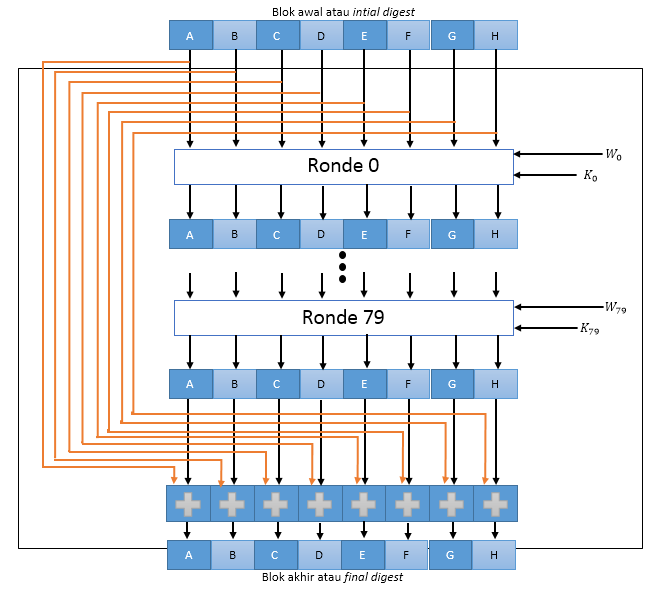
\includegraphics[scale=0.7]{Gambar/compression_function}
	\centering
	\caption{Struktur Putaran dalam SHA-512}\label{fig:strukturputaran}
\end{figure}

Dalam 1 putaran SHA-512, \textit{word} keluaran diperoleh dari salinan word \textit{masukan}, berikut menunjukkan masukan dan keluaran dari masing-masing \textit{word}.

\begin{itemize}
	\item \textit{Word} keluaran \textit{B} diperoleh dari \textit{word} masukan \textit{A}
	\item \textit{Word} keluaran \textit{C} diperoleh dari \textit{word} masukan \textit{B}
	\item \textit{Word} keluaran \textit{D} diperoleh dari \textit{word} masukan \textit{C}
	\item \textit{Word} keluaran \textit{F} diperoleh dari \textit{word} masukan \textit{E}
	\item \textit{Word} keluaran \textit{G} diperoleh dari \textit{word} masukan \textit{F}
	\item \textit{Word} keluaran \textit{H} diperoleh dari \textit{word} masukan \textit{G}
\end{itemize}

Gambar \ref{fig:masukankeluaranword} menunjukkan ilustrasi dari masukan dan keluaran dalam 1 putaran SHA-512 untuk setiap \textit{word}.

%diagram
\begin{figure}[H]
	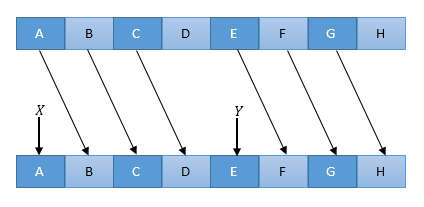
\includegraphics[scale=0.8]{Gambar/sha_round}
	\centering
	\caption{Masukan dan Keluaran dalam 1 Putaran SHA-512}\label{fig:masukankeluaranword}
\end{figure}

Untuk nilai \textit{word} keluaran \textit{A} dan \textit{E} diperoleh dari \textit{word} \textit{X} dan \textit{Y}. \textit{Word} \textit{X} dan \textit{Y} ini diperoleh dari sebuah fungsi khusus. Gambar \ref{fig:fungsikhusus} menunjukkan struktur dari fungsi khusus. Berikut akan dijelaskan struktur dari fungsi khusus.

\subsubsection{Struktur Fungsi Khusus}

%diagram
\begin{figure}[H]
	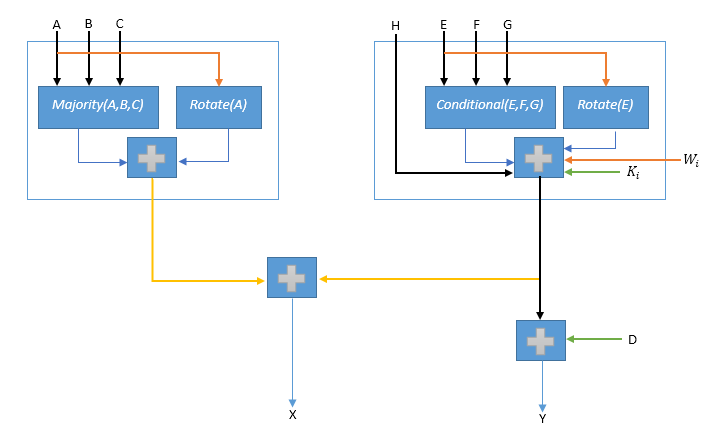
\includegraphics[scale=0.7]{Gambar/complex_function}
	\centering
	\caption{Fungsi Khusus dalam 1 Putaran SHA-512}\label{fig:fungsikhusus}
\end{figure}

\textit{Word Y} pada gambar \ref{fig:fungsikhusus} diperoleh dari proses persamaan \ref{eq:fungsikhusus1}.

\begin{equation}
	Y = D + (Conditional(E,F,G) + Rotate(E) + W_i + K_i + H) \label{eq:fungsikhusus1}
\end{equation}

Nilai \begin{math}W_i\end{math} diperoleh dari proses Ekspansi Blok \textit{Message} (Subbab \ref{subsec:expansiblokmsg}), dimana \textit{i} menunjukkan urutan dari putaran. Nilai \begin{math}K_i\end{math} pada persamaan \ref{eq:fungsikhusus1} diperoleh dari nilai belakang koma akar kubik bilangan prima ke-\begin{math}(i+1)\end{math}. Kemudian, nilai belakang koma ini akan dikonversi menjadi heksadesimal. 

Bilangan prima yang digunakan untuk menghitung nilai \begin{math}K_i\end{math} dimulai dari 2 untuk \begin{math}K_0\end{math}, 3 untuk \begin{math}K_1\end{math}, dan seterusnya secara berurutan sampai 409 untuk \begin{math}K_{79}\end{math}. Persamaan \ref{eq:fungsikhusus2} menunjukkan cara untuk menghitung salah satu dari nilai \begin{math}K_i\end{math}.

\begin{gather}
	K_{79} = \sqrt[3]{409} \nonumber \\
	= 7.4229141204362155 \nonumber \\
	= (7.6C44198C4A475817)_{16} \label{eq:fungsikhusus2} \\
	= 6C44198C4A475817 \nonumber
\end{gather}

Sementara itu, untuk operasi \textit{Conditional} pada persamaan \ref{eq:fungsikhusus1} adalah operasi \textit{AND}, \textit{OR} dan \textit{XOR} dari \textit{bit-bit} setiap \textit{word}. Rumus dari \textit{Conditional} ditunjukkan oleh persamaan \ref{eq:fungsikhusus3}.

\begin{equation}
	Conditional(x,y,z) = (x\: AND\: y) \oplus (NOT\: x\: AND\: z) \label{eq:fungsikhusus3}
\end{equation}

Operasi \textit{Rotate} pada persamaan \ref{eq:fungsikhusus1} adalah hasil \textit{exclusive-or} (XOR) dari \begin{math}RotR_i(x)\end{math}. \begin{math}RotR_i(x)\end{math} merupakan operasi rotasi ke kanan \textit{x} sebanyak \textit{i-bit} yang sudah dijelaskan pada proses Ekspansi Blok Message (Subbab \ref{subsec:expansiblokmsg}). Rumus dari \textit{Rotate} ditunjukkan pada persamaan \ref{eq:fungsikhusus4}.

\begin{equation}
	Rotate(x) = RotR_{28}(x) \oplus RotR_{34}(x) \oplus RotR_{39}(x) \label{eq:fungsikhusus4}
\end{equation}

Hasil pertambahan \textit{bit-bit} operasi \textit{Conditional}, operasi \textit{Rotate}, \begin{math}W_i\end{math}, \begin{math}K_i\end{math}, dan \textit{word} \begin{math}H\end{math} akan ditambahkan dengan \textit{word} \begin{math}D\end{math} untuk menghasilkan \textit{word} \begin{math}Y\end{math}.

Kemudian, \textit{word} \begin{math}X\end{math} pada Gambar \ref{fig:fungsikhusus} diperoleh dari persamaan \ref{eq:fungsikhusus5}.

\begin{equation}
	X = (Majority(A,B,C) + Rotate(A)) + (Conditional(E,F,G) + Rotate(E) + W_i + K_i + H) \label{eq:fungsikhusus5}
\end{equation}

Untuk operasi \textit{Conditional} dan \textit{Rotate} sudah dijelaskan pada persamaan \ref{eq:fungsikhusus3} dan \ref{eq:fungsikhusus3}. Sementara itu, untuk operasi \textit{Majority} pada persamaan \ref{eq:fungsikhusus5} adalah operasi \textit{AND}, \textit{OR} dan \textit{XOR} dari \textit{bit-bit} setiap \textit{word}. Operasi \textit{Majority} ditunjukkan pada persamaan \ref{eq:fungsikhusus6}.

\begin{equation}
	Majority(x,y,z) = (x\: AND\: y) \oplus (y\: AND\: z) \oplus (z\: AND\: x) \label{eq:fungsikhusus6}
\end{equation}

Hasil akhir dari fungsi khusus adalah \textit{word} \begin{math}X\end{math} dan \textit{word} \begin{math}Y\end{math}. \textit{Word} \begin{math}X\end{math} akan menjadi \textit{word} keluaran \begin{math}A\end{math} dan \textit{word} \begin{math}Y\end{math} akan menjadi \textit{word} keluaran \begin{math}E\end{math}. Ilustrasi dari hasil keluaran ini ditunjukkan oleh Gambar \ref{fig:masukankeluaranword}.

Proses setelah 80 putaran dilakukan adalah operasi pertambahan masing-masing \textit{bit} dari blok 512-\textit{bit} hasil keluaran putaran ke-80 dengan masing-masing \textit{bit} dari blok 512-\textit{bit} masukan untuk putaran ke-1. Ilustrasi proses ini ditunjukkan oleh Gambar \ref{fig:compression_function}. 

Kemudian, hasil akhir dari proses tersebut berupa blok dengan panjang 512-\textit{bit} terdiri dari 8 \textit{word}. Blok 512-\textit{bit} ini akan menjadi hasil akhir (\textit{digest}) atau menjadi masukan untuk fungsi kompresi yang digunakan oleh blok \textit{message} ke-2 dan seterusnya. Gambar \ref{fig:digestcreate} menunjukkan proses yang sudah dijelaskan.

%diagram
\begin{figure}[H]
	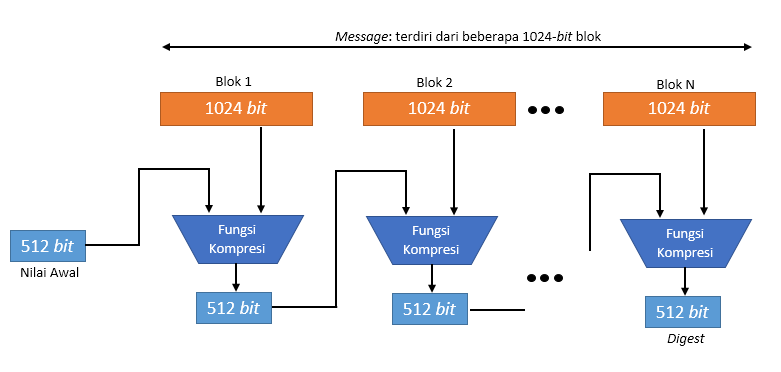
\includegraphics[scale=0.7]{Gambar/digest_creation}
	\caption{Proses Keseluruhan dari SHA-512}\label{fig:digestcreate}
\end{figure}

\section{Otentikasi}

Otentikasi adalah proses untuk menentukan keaslian identitas dari sebuah entitas saat akan mengakses sumber daya sebuah sistem. Berdasarkan entitas yang diotentikasi \cite{forouzan2007cryptography}, otentikasi dibagi menjadi 2 jenis, yaitu:

\begin{enumerate}
	\item Otentikasi pesan \\
	Otentikasi pesan adalah proses otentikasi untuk memastikan bahwa pesan berasal dari sumber data yang bisa dipercaya. Otentikasi pesan juga memastikan bahwa pesan tidak diubah saat pengiriman pesan sedang berlangsung. Beberapa teknik otentikasi pesan adalah \textit{Modification Detection Code} dan \textit{Message Authentication Code}.
	\item Otentikasi entitas \\
	Otentikasi entitas adalah proses otentikasi untuk memastikan kebenaran identitas seseorang. Entitas yang diotentikasi bisa berupa orang atau pengguna (\textit{user}). Beberapa teknik otentikasi entitas adalah \textit{password}, \textit{zero-knowledge}, \textit{challenge-response}, dan biometrik.
\end{enumerate}

Sementara itu, berdasarkan bentuknya\cite{forouzan2007cryptography}, otentikasi dibagi menjadi 3 jenis, yaitu:
\begin{enumerate}
	\item Sesuatu yang diketahui (\textit{something known}) \\
	Sesuatu yang diketahui oleh pengirim pesan dan kebenarannya bisa dipastikan oleh penerima pesan. Contohnya antara lain adalah \textit{password}, nomor PIN, \textit{passphrase}, dan sebagainya.
	\item Sesuatu yang dimiliki (\textit{something possessed}) \\
	Sesuatu yang dimiliki adalah sesuatu yang menunjukkan identitas dari pengirim pesan. Contohnya adalah paspor, KTP, kartu kredit, SIM, dan sebagainya.
	\item Sesuatu yang melekat (\textit{something inherent}) \\
	Sesuatu yang melekat adalah sesuatu yang menempel atau sebagai bagian dari pengirim pesan. Contohnya adalah sidik jari, suara, pola retina, dan sebagainya.
\end{enumerate}

\subsection{\textit{Password}}

\textit{Password} adalah sekumpulan huruf, angka, dan simbol yang sifatnya rahasia. \textit{Password} merupakan salah satu teknik dari otentikasi entitas. \textit{Password} digunakan saat seseorang hendak mengakses sumber daya sebuah sistem, seperti \textit{email}, akun media sosial, dan sebagainya. \textit{Password} ini sifatnya rahasia dan tidak boleh diketahui oleh pihak yang tidak berhak.

Berdasarkan cara penggunaannya\cite{forouzan2007cryptography}, password dibagi menjadi 2 jenis, yaitu:
\begin{enumerate}
	\item \textit{One-Time Password} \\
	\textit{One-Time Password} adalah \textit{password} yang digunakan hanya satu kali untuk setiap akses kepada sistem. Jadi, setiap kali pengguna mengakses sistem dalam sesi waktu yang berbeda, \textit{password} yang digunakan pun akan berbeda-beda. Beberapa contoh dari \textit{One-Time Password} adalah \textit{List of Passwords, Sequentially Updated Password,} dan \textit{Lamport One-Time Password}.
	\item \textit{Password} Tetap \\
	\textit{Password} tetap adalah \textit{password} yang digunakan berulang-ulang setiap kali pengguna akan mengakses sistem. \textit{Password} yang digunakan untuk mengakses sistem selalu sama. Berikut adalah beberapa skema dari \textit{password} tetap.
\end{enumerate}

\subsubsection{Skema 1}

Dalam skema ini, sistem menyimpan setiap \textit{password} pada sebuah tabel basis data. \textit{Password} yang disimpan di tabel basis data berupa \textit{plaintext}, artinya bisa dibaca dan dimengerti. Masing-masing dari \textit{password} memiliki \textit{username} yang disimpan juga di tabel basis data. Saat pengguna akan mengakses sistem, pengguna akan memasukan \textit{username} dan \textit{password}.

Kemudian, saat pengguna sudah memasukan \textit{username} dan \textit{password}, sistem akan mencari informasi dari pengguna di tabel basis data lewat \textit{username}. Karena setiap \textit{username} memiliki \textit{password}, sistem akan menyesuaikan \textit{username} dan \textit{password} di tabel basis data dengan \textit{username} dan \textit{password} yang dimasukan oleh pengguna saat hendak mengakses sistem. Jika \textit{username} dan \textit{password} yang dimasukan pengguna sesuai dengan \textit{username} dan \textit{password} di tabel basis data maka hak akses sistem akan diberikan. Gambar \ref{fig:password1} menunjukkan proses yang dijelaskan.

% diagram
\begin{figure}[H]
	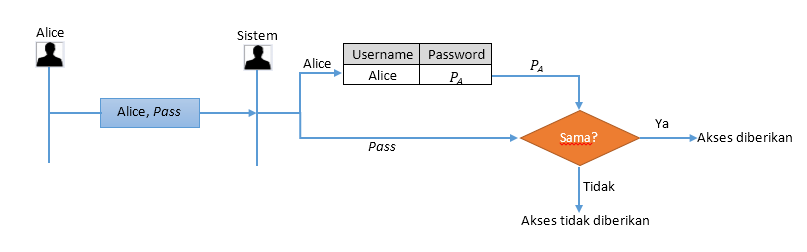
\includegraphics[scale=0.7]{Gambar/password_1}
	\centering
	\caption{\textit{Username} dan \textit{Password}}\label{fig:password1}
\end{figure}

Kelebihan dari skema ini adalah skema ini mudah untuk diimplementasikan dan tidak membutuhkan proses yang rumit. Sementara itu, kekurangan dari skema ini adalah \textit{password} yang disimpan di tabel basis data bisa dibaca dan dimengerti karena disimpan dalam bentuk \textit{plaintext}. Akibatnya, jika ada pihak yang tidak memiliki hak akses berhasil memperoleh \textit{password} yang disimpan di tabel basis data, maka \textit{password} sudah tidak rahasia lagi.

\subsubsection{Skema 2}

Dalam skema ini, sistem tetap menyimpan \textit{username} dan \textit{password} dalam tabel basis data. \textit{Password} yang disimpan tidak dalam bentuk \textit{plaintext}nya, tetapi disimpan dalam bentuk \textit{digest}nya. Saat pengguna hendak mengakses sistem, pengguna tetap memasukan \textit{username} dan \textit{password} dalam bentuk \textit{plaintext}.

Kemudian, saat pengguna sudah memasukan \textit{username} dan \textit{password}, sistem akan terlebih dahulu menghitung \textit{digest} dari \textit{password} yang dimasukan menggunakan fungsi \textit{hash}. Setelah itu, \textit{username} dan \textit{digest} akan disesuaikan dengan \textit{username} dan \textit{digest} yang disimpan dalam tabel basis data. Jika sesuai, maka pengguna akan diberikan hak akses ke sistem. Gambar \ref{fig:password2} menunjukkan proses yang sudah dijelaskan.

% diagram
\begin{figure}[H]
	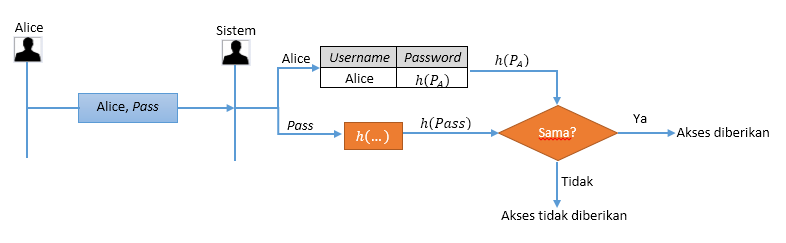
\includegraphics[scale=0.7]{Gambar/password_2}
	\centering
	\caption{\textit{Password hashing}}\label{fig:password2}
\end{figure}

Kelebihan dari skema ini adalah walaupun \textit{password} yang disimpan dalam tabel basis data diketahui oleh pihak yang tidak berhak, \textit{password} tidak akan bisa dimengerti karena disimpan dalam bentuk \textit{digest}nya. Sementara itu, \textit{digest} tidak bisa dikembalikan ke dalam bentuk \textit{plaintext} untuk mendapatkan \textit{password} karena fungsi \textit{hash} adalah fungsi satu arah seperti yang sudah dibahas dalam \ref{sec:fungsihash}. Sementara itu, kekurangan dari skema ini adalah \textit{digest} yang disimpan masih rentan terhadap \textit{dictionary attack}. Penjelasan tentang \textit{dictionary attack} akan dijelaskan pada skema selanjutnya.

\subsubsection{Skema 3}

Dalam skema 3, sistem tetap menyimpan \textit{username}. Password juga disimpan dalam bentuk \textit{digest}nya. Dalam skema ini, sebelum \textit{digest password} dibuat, \textit{password} akan dikonkatenasi dengan \textit{salt}. \textit{Salt} adalah sebuah \textit{string} acak yang bisa berisi angka, huruf, atau simbol.

Penggunaan \textit{salt} disini bertujuan untuk mengurangi tingkat keberhasilan \textit{dictionary attack}. \textit{Dictionary attack} adalah serangan dengan mencoba semua kemungkinan \textit{string} masukan untuk fungsi \textit{hash} sampai menghasilkan \textit{digest} yang sesuai. Dengan adanya penambahan \textit{salt}, maka akan mengurangi kemungkinan keberhasilan dari \textit{dictionary attack} karena banyak kemungkinan dari \textit{string} masukan akan bertambah sehingga semakin sulit untuk mendapatkan \textit{digest} yang sesuai.

Karena \textit{salt} dibutuhkan untuk mengurangi tingkat keberhasilan \textit{dictionary attack}, nilai \textit{salt} akan disimpan juga dalam tabel basis data. Kemudian, saat pengguna sudah memasukan \textit{username} dan \textit{password}, sistem akan menerima \textit{password} yang dimasukan. Selanjutnya, \textit{password} dikonkatenasi dengan \textit{salt} yang disimpan lalu sistem akan menghitung \textit{digest} dari hasil konkatenasi \textit{password} dengan \textit{salt}. Setelah itu, sistem akan membandingkan dengan \textit{digest} yang disimpan dalam tabel basis data. Jika sesuai, pengguna akan diberikan hak akses ke sistem. Gambar \ref{fig:password3} menunjukkan proses yang dijelaskan.

% diagram
\begin{figure}[H]
	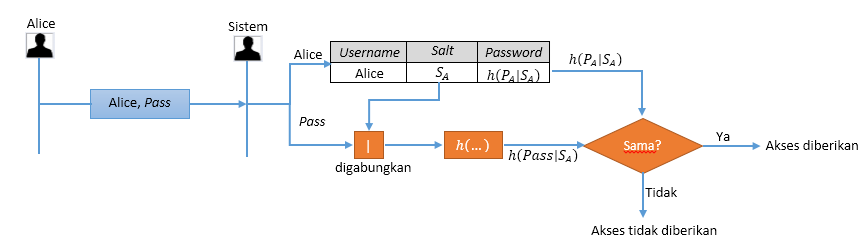
\includegraphics[scale=0.7]{Gambar/password_3}
	\centering
	\caption{\textit{Password salting}}\label{fig:password3}
\end{figure}

Kelebihan dari skema ini adalah \textit{password} tidak akan bisa diketahui dengan mudah lewat \textit{dictionary attack}. Banyak kemungkinan digest yang semakin bertambah menyebabkan serangan dengan \textit{dictionary attack} semakin sulit. Sementara itu, kekurangan dari skema ini adalah rumit karena membutuhkan banyak proses hanya untuk memberikan akses.

\section{Eliminasi Gauss-Jordan}\label{sec:eliminasigaussjordan}

Eliminasi Gauss-Jordan adalah suatu metode untuk menyelesaikan sistem persamaan linear dengan mereduksi matriks menjadi eselon baris tereduksi\cite{norman2012introduction}. Suatu matriks \begin{math}R\end{math} dikatakan bentuk eselon baris tereduksi jika memenuhi syarat sebagai berikut\cite{norman2012introduction}.

\begin{enumerate}
	\item Terdapat baris yang tidak seluruhnya terdiri dari angka 0 \\
	Angka bukan 0 pertama dari sebelah kiri dari baris tersebut disebut 1 utama.
	\item Baris yang seluruhnya terdiri dari angka 0 harus menjadi baris paling bawah.
	\item Pada kolom 1 utama, seluruh angka di bawah 1 utama harus 0.
\end{enumerate}

Sebagai contoh, matriks-matriks eselon baris tereduksi ditunjukkan oleh Matriks \ref{eq:gaussmatriks1}.

\begin{center}
	\setlength\arraycolsep{10pt}
	\begin{gather}
		\begin{bmatrix}
				1 	& 12 	& 5 	& 4 		\\[1em]
				0 	& 2 	& 4 	& 8 		\\[1em]
				0 	& 0 	& 9 	& 3
		\end{bmatrix},
		\begin{bmatrix}
				1 & 0 	\\[1em]
				0 & 1
		\end{bmatrix},
		\begin{bmatrix}
				1 	& 0 	& 2 	& 5 		\\[1em]
				0 	& 5 	& 4 	& 8 		\\[1em]
				0 	& 0 	& 4 	& 10		\\[1em]
				0 	& 0 	& 0 	& 0
		\end{bmatrix} \label{eq:gaussmatriks1}
	\end{gather}
\end{center}

Proses eliminasi Gauss-Jordan dibagi menjadi 2 proses, yaitu proses mereduksi matriks menjadi bentuk eselon baris dan proses substitusi balik ke sistem persamaan linear untuk memperoleh solusi sistem persamaan linear. Dimisalkan sistem persamaan linear yang akan dicari solusinya ditunjukkan oleh persamaan \ref{eq:gaussmatriks0}. Berikut akan dijelaskan proses mereduksi matriks menjadi bentuk eselon baris.

\begin{gather}
	x + y + z = 10 \nonumber \\
	x + 2y + 4z = 21 \label{eq:gaussmatriks0} \\
	x + 3y + 9z = 38 \nonumber
\end{gather}

\subsection{Proses Reduksi Matriks}

Proses mereduksi matriks menjadi eselon baris dilakukan dengan cara operasi baris. Operasi baris adalah suatu metode untuk mereduksi matriks menjadi eselon baris dengan cara sebagai berikut.

\begin{enumerate}
	\item Mengalikan baris dengan konstanta selain 0.
	\item Menukar 2 baris.
	\item Mengurangi sebuah baris dengan baris lainnya.
\end{enumerate}

Langkah paling awal adalah mengubah persamaan \ref{eq:gaussmatriks0} menjadi matriks. Konstanta dari variabel ke-$i$ dari persamaan ke-$j$ akan menjadi elemen matriks kolom ke-$i$ dan baris ke-$j$. Sebagai contoh, variabel ke-1 dan persamaan ke-1 dari persamaan \ref{eq:gaussmatriks0} adalah $x$ dengan konstanta 1, maka elemen matriks kolom ke-1 baris ke-1 adalah 1. Contoh lainnya, variabel ke-2 dan persamaan ke-3 persamaan \ref{eq:gaussmatriks0} adalah $3y$ dengan konstanta 3, maka elemen matriks kolom ke-2 baris ke-3 adalah 3. Hasil pengubahan persamaan \ref{eq:gaussmatriks0} menjadi matriks ditunjukkan oleh Matriks \ref{eq:gaussmatriks2}.

\begin{center}
	\setlength\arraycolsep{10pt}
	\begin{equation}
		\begin{bmatrix}
				1 	& 1 	& 1 	& 10 		\\[1em]
				1 	& 2 	& 4 	& 21 		\\[1em]
				1 	& 3 	& 9 	& 38
		\end{bmatrix} \label{eq:gaussmatriks2}
	\end{equation}
\end{center}

Operasi baris pertama adalah mengurangi baris ke-3 dan baris ke-2 dengan baris ke-1. Maka, hasil pengurangan baris ditunjukkan oleh Matriks \ref{eq:gaussmatriks3}.

\begin{center}
	\setlength\arraycolsep{10pt}
	\begin{equation}
		\begin{bmatrix}
				1 			& 1 		& 1 		& 10 				\\[1em]
				1 - 1 	& 2 - 1	& 4 - 1	& 21 - 10		\\[1em]
				1 - 1		& 3 - 1	& 9 - 1	& 38 - 10
		\end{bmatrix} \Rightarrow
		\begin{bmatrix}
				1 	& 1 	& 1 	& 10 		\\[1em]
				0 	& 1 	& 3 	& 11 		\\[1em]
				0 	& 2 	& 8 	& 28
		\end{bmatrix} \label{eq:gaussmatriks3}
	\end{equation}
\end{center}

Kemudian, operasi baris kedua adalah mengurangi baris ke-3 dengan baris ke-2 yang dikali dengan konstanta 2. Hasil operasi baris kedua ditunjukkan oleh Matriks \ref{eq:gaussmatriks4}.

\begin{center}
	\setlength\arraycolsep{10pt}
	\begin{equation}
		\begin{bmatrix}
				1 	& 1 							& 1 							& 10 		\\[1em]
				0 	& 1 							& 3 							& 11 		\\[1em]
				0 	& 2 - (1\cdot2) 	& 8 - (3\cdot2) 	& 28 - (11\cdot2)
		\end{bmatrix} \Rightarrow
		\begin{bmatrix}
				1 	& 1 	& 1 	& 10 		\\[1em]
				0 	& 1 	& 3 	& 11 		\\[1em]
				0 	& 0 	& 2 	& 6
		\end{bmatrix} \label{eq:gaussmatriks4}
	\end{equation}
\end{center}

Setelah operasi baris kedua, maka diperoleh Matriks \ref{eq:gaussmatriks5} yang merupakan matriks dengan bentuk eselon baris tereduksi.

\begin{center}
	\setlength\arraycolsep{10pt}
	\begin{equation}
		\begin{bmatrix}
				1 	& 1 	& 1 	& 10 		\\[1em]
				0 	& 1 	& 3 	& 11 		\\[1em]
				0 	& 0 	& 2 	& 6
		\end{bmatrix} \label{eq:gaussmatriks5}
	\end{equation}
\end{center}

\subsection{Proses Substitusi Balik}

Setelah mengubah matriks menjadi bentuk eselon baris tereduksi, proses substitusi balik adalah proses untuk mencari nilai koefesien dari masing-masing variabel untuk memperoleh solusi dari persamaan linear \ref{eq:gaussmatriks0}. Kolom paling kanan (kolom ke-\begin{math}n\end{math}) dari matriks menunjukkan nilai solusi dari masing-masing baris. Sementara itu, kolom ke-1 sampai kolom ke-(\begin{math}n-1\end{math}) menunjukkan koefesien dari persamaan linear.

Sebagai contoh, dari Matriks \ref{eq:gaussmatriks5} diperoleh hasilnya sebagai berikut.

\begin{gather}
	2z = 6 \nonumber \\
	z = 3 \label{eq:gaussmatriks6}
\end{gather}

Kemudian, untuk nilai \begin{math}y\end{math}.

\begin{gather}
	y + 3z = 11 \nonumber \\
	y + 3\cdot3 = 11 \nonumber \\
	y + 9 = 11 \nonumber \\
	y = 2 \label{eq:gaussmatriks7}
\end{gather}

Kemudian, untuk nilai \begin{math}x\end{math}.

\begin{gather}
	x + y + z = 10 \nonumber \\
	x + 2 + 3 = 10 \nonumber \\
	x + 5 = 10 \nonumber \\
	x = 5 \label{eq:gaussmatriks8}
\end{gather}

Jadi, solusi dari persamaan \ref{eq:gaussmatriks0} yang diselesaikan dengan eliminasi Gauss-Jordan adalah \begin{math}x=5, y=2,\end{math} dan \begin{math}z=3\end{math}.

\section{\textit{Secret Sharing} Shamir}\label{sec:secretsharingshamir}

Pada bagian ini akan dijelaskan mengenai sejarah singkat yang mengawali munculnya secret sharing Shamir dan pembahasan mengenai secret sharing Shamir.

\subsection{Sejarah Singkat}

\textit{Secret sharing} adalah metode untuk membagi informasi (rahasia) menjadi beberapa bagian. Bagian-bagian tersebut disebut \textit{share} dan setiap bagian dibagikan kepada beberapa partisipan. Untuk mendapatkan kembali informasi, maka dibutuhkan setiap \textit{share}.

Permasalahan muncul jika share dan partisipan bertambah banyak. Proses untuk mendapatkan kembali rahasia akan menjadi sulit karena setiap share harus ada. Karena permasalahan ini, pada tahun 1979 Adi Shamir memublikasikan pengembangan dari metode \textit{secret sharing} dalam esai yg berjudul '\textit{How to Share a Secret}'\cite{shamir1979share}. Metode yang dikembangkan Adi Shamir dinamakan \textit{secret sharing} Shamir.

\subsection{Pembahasan \textit{Secret Sharing} Shamir}

Untuk mengatasi permasalahan yang sudah dibahas, Shamir mengubah cara untuk mendapatkan kembali informasi. Misalkan, informasi dilambangkan dengan data \textit{D}. Dalam metode \textit{secret sharing} Shamir data \textit{D} yang dibagi menjadi \begin{math}n\end{math} \textit{share} hanya memerlukan minimal \begin{math}k\end{math} \textit{share} untuk memperoleh kembali \begin{math}D\end{math}. Skema yang dikembangkan Shamir ini dinamakan skema \textit{threshold}(\textit{k},\textit{n}),

\subsubsection{Skema \textit{Threshold}(\textit{k},\textit{n})}

Skema \textit{threshold}(\textit{k},\textit{n}) adalah skema \textit{secret sharing} dimana hanya minimal \textit{k} \textit{share} dari \textit{n} \textit{share} dibutuhkan untuk mengembalikan data \textit{D}. Skema ini memiliki ketentuan sebagai berikut\cite{shamir1979share}.

\begin{itemize}
	\item Jika \textit{share} yang dimiliki sebanyak \textit{k} \textit{share} atau lebih, \textit{D} bisa dibentuk kembali.
	\item Jika \textit{share} yang ada hanya sebanyak \textit{k-1} atau kurang maka \textit{D} tidak bisa dibentuk kembali.
\end{itemize}

Ada 2 proses dalam skema \textit{threshold}(\textit{k},\textit{n}), yaitu proses pembangunan \textit{share} dari rahasia dan proses rekonstruksi rahasia dari \textit{share} yang dimiliki. Dimisalkan rahasia adalah \begin{math}D\end{math}. Proses pertama adalah proses pembangunan \textit{share} dari \begin{math}D\end{math}. Berikut akan dijelaskan proses pembangunan \textit{share}.

\subsubsection{Proses Pembangunan \textit{Share}}

Langkah pertama adalah memilih nilai \begin{math}k\end{math}. Kemudian, setelah memilih nilai \begin{math}k\end{math} langkah selanjutnya adalah membentuk \begin{math}k-1\end{math} derajat fungsi \begin{math}f(x)\end{math}. Persamaan \ref{eq:secretsharing1} menunjukkan fungsi \begin{math}f(x)\end{math} yang dibentuk.

\begin{equation}
	f(x) = a_0 + a_1x + a_2x^2 + ... + a_{k-1}x^{k-1} \label{eq:secretsharing1}
\end{equation}

\begin{flushleft}
	dimana \begin{math}a_0 = D\end{math}.
\end{flushleft}

Setelah membentuk fungsi \begin{math}f(x)\end{math}, langkah selanjutnya adalah memilih banyak share, yaitu nilai \begin{math}n\end{math}. Setelah memilih \begin{math}n\end{math}, \begin{math}x=1\end{math} sampai \begin{math}x=n\end{math} akan dipetakan dengan fungsi \begin{math}f(x)\end{math} untuk memperoleh \begin{math}D_i\end{math}. Persamaan \ref{eq:secretsharing2} menunjukkan hasil pemetaan dengan fungsi \begin{math}f(x)\end{math}.

\begin{equation}
	D_1 = f(1), D_2 = f(2), ..., D_i = f(i), ..., D_n = f(n) \label{eq:secretsharing2}
\end{equation}

Nilai \begin{math}D_1\end{math} sampai \begin{math}D_n\end{math} adalah \textit{share} dari data \begin{math}D\end{math}.

\subsubsection{Proses Rekonstruksi Rahasia}

Pada bagian ini akan dijelaskan proses rekonstruksi \begin{math}D\end{math} dari \begin{math}D_1, D_2, ..., D_n\end{math} yang sudah dibangun dalam Proses Pembangunan \textit{Share}. Langkah pertama adalah membentuk membentuk \begin{math}k-1\end{math} derajat fungsi \begin{math}f(x)\end{math} dari \begin{math}k\end{math} yang sudah dipilih dalam Proses Pembangunan \textit{Share}. Persamaan \ref{eq:secretsharing3} menunjukkan fungsi \begin{math}f(x)\end{math} yang dibentuk.

\begin{equation}
	f(x) = a_0 + a_1x + a_2x^2 + ... + a_{k-1}x^{k-1} \label{eq:secretsharing3}
\end{equation}

Setelah itu, langkah selanjutnya adalah membentuk \begin{math}k\end{math} fungsi \begin{math}f(x)\end{math} dengan memetakan \begin{math}k\end{math} \textit{share} yang dimiliki dengan fungsi \begin{math}f(x)\end{math}. Hasil pemetaan dengan fungsi \begin{math}f(x)\end{math} ini adalah \textit{share} yang sudah dibangun pada Proses Pembangunan \textit{Share}. Persamaan \ref{eq:secretsharing4} menunjukkan hasil pemetaan masing-masing fungsi \begin{math}f(x)\end{math}.

\begin{gather}
	f(1) = a_0 + a_1\cdot 1 + a_2\cdot 1^2 + ... + a_{k-1}\cdot 1^{k-1} = D_1 \nonumber \\
	f(2) = a_0 + a_1\cdot 2 + a_2\cdot 2^2 + ... + a_{k-1}\cdot 2^{k-1} = D_2 \nonumber \\
	\vdots \nonumber \\
	f(k) = a_0 + a_1\cdot k + a_2\cdot k^2 + ... + a_{k-1}\cdot k^{k-1} = D_k \label{eq:secretsharing4}
\end{gather}

Dari hasil pemetaan yang ditunjukkan persamaan \ref{eq:secretsharing4}, langkah selanjutnya adalah membentuk persamaan linear. persamaan \ref{eq:secretsharing5} menunjukkan persamaan linear yang dibentuk.

\begin{gather}
	a_0 + a_1\cdot 1 + a_2\cdot 1^2 + ... + a_{k-1}\cdot 1^{k-1} = D_1 \qquad...\text{\textcircled{1}} \nonumber \\
	a_0 + a_1\cdot 2 + a_2\cdot 2^2 + ... + a_{k-1}\cdot 2^{k-1} = D_2 \qquad...\text{\textcircled{2}} \nonumber \\
	\vdots \nonumber \\
	a_0 + a_1\cdot k + a_2\cdot k^2 + ... + a_{k-1}\cdot k^{k-1} = D_k \qquad...\text{\textcircled{k}} \label{eq:secretsharing5}
\end{gather}

Setelah membentuk persamaan linear, langkah selanjutnya adalah menyelesaikan persamaan linear tersebut dengan metode Eliminasi Gauss-Jordan yang sudah dijelaskan pada Subbab \ref{sec:eliminasigaussjordan}. Tujuannya adalah untuk memperoleh nilai \begin{math}a_1, a_2, ..., a_{k-1}\end{math}. Dengan menggunakan Proses Substitusi Balik dalam metode Eliminasi Gauss-Jordan, dapat diperoleh nilai \begin{math}a_0\end{math} yang adalah data \begin{math}D\end{math}.

\section{Probabilitas}
Probabilitas atau peluang merupakan salah cara dalam ilmu matematika untuk mengukur tingkat kepercayaan akan suatu kejadian. Teori probabilitas sangat luas penggunaannya, baik dalam kehidupan sehari-hari maupun dalam percobaan-percobaan ilmiah. Teori probabilitas ini seringkali digunakan oleh para pengambil keputusan untuk memprediksi suatu kejadian sehingga nantinya bisa mengambil keputusan yang tepat.

Seluruh kemungkinan keluaran yang akan terjadi dalam probabilitas disebut ruang sampel sedangkan masing-masing kemungkinan yang dapat terjadi dalam ruang sampel dinamakan elemen kejadian atau anggota dari ruang sampel. Ruang sampel dilambangkan dengan huruf \begin{math}S\end{math} dan elemen kejadian dilambangkan dengan huruf \begin{math}x_i\end{math}. Dalam ruang sampel \begin{math}S\end{math} dengan \begin{math}i\end{math} elemen kejadian, ditunjukkan pada persamaan \ref{eq:probability1}.

\begin{equation}
	S = {x_1, x_2, x_3, ..., x_i}
	\label{eq:probability1}
\end{equation}

Sedangkan probabilitas kejadian \begin{math}x_i\end{math} akan terjadi dilambangkan dengan \begin{math}P(x_i)\end{math}. Maka, rumus matematikanya ditunjukkan pada persamaan \ref{eq:probability2}.

\begin{equation}
	P(x_i) = \frac{n}{N}
	\label{eq:probability2}
\end{equation}

\noindent dimana \begin{math}n\end{math} adalah banyaknya kemunculan kejadian \begin{math}x_i\end{math} dalam sebuah ruang sampel \begin{math}S\end{math} dan \begin{math}N\end{math} adalah banyaknya kejadian yang terjadi dalam ruang sampel \begin{math}S\end{math}.

\subsection{Distribusi Binom}

Setiap eksperimen atau percobaan yang dilakukan secara berkali-kali pasti memiliki dua keluaran, yaitu sukses atau gagal. Untuk setiap keluaran yang diperoleh (baik sukses maupun gagal) bisa ditetapkan sebagai sukses. Proses ini dinamakan proses Bernouli dan setiap eksperimen yang dilakukan untuk setiap proses bernouli dinamakan percobaan Bernouli. Ada beberapa syarat sebuah eksperimen bisa dinamakan percobaan Bernouli\cite{walpole1993probability}:
\begin{enumerate}
	\item Eksperimen harus diulang sebanyak \begin{math}n\end{math} kali.
	\item Hasil keluaran setiap perulangan hanya 2 kemungkinan, yaitu keluaran sukses atau keluaran gagal.
	\item Hasil keluaran setiap perulangan tidak mempengaruhi dengan perulangan yang lain.
	\item Probabilitas bahwa hasil keluarannya sukses, \begin{math}p\end{math}, harus selalu sama untuk setiap kali perulangan.
\end{enumerate}

Percobaan Bernouli digunakan untuk menghitung probabilitas \begin{math}x\end{math} buah hasil keluaran yang sukses dari \begin{math}n\end{math} percobaan. Dimisalkan bahwa probabilitas hasil keluaran setiap perulangan sukses adalah \begin{math}p\end{math}. Sebaliknya, probabilitas hasil keluaran setiap perulangan gagal adalah \begin{math}q=1-p\end{math}. Persamaan \ref{eq:binom} untuk menghitung probabilitas \begin{math}x\end{math} hasil keluaran yang sukses dari \begin{math}n\end{math} percobaan.

\begin{gather}
	P(x,n,p) = \left( {\begin{array}{c}n \\ x \end{array}} \right) p^x q^{n-x} \label{eq:binom} \\
	x = 0, 1, 2, ..., n \nonumber
\end{gather}

\begin{math}\left( {\begin{array}{c}n \\ x \end{array}} \right)\end{math} pada persamaan \ref{eq:binom} menunjukkan bahwa dari \begin{math}n\end{math} percobaan akan dipilih \begin{math}x\end{math} hasil keluaran yang sukses.

\section{Entropi}

Pada bagian ini akan dijelaskan mengenai entropi dimulai dari sejarah singkat entropi dan pembahasan mengenai entropi.

\subsection{Sejarah Singkat}

Istilah entropi muncul pertama kali dalam esai '\textit{A Mathematical Theory of Communication}' pada tahun 1948. Esai ini dibuat oleh Claude E. Shannon seorang ilmuwan asal Amerika Serikat. Dalam esainya, Shannon menulis bahwa entropi adalah konsep keacakan atau suatu ketidakpastian\cite{shannon1948mathematical}. Istilah dari entropi ini dinamakan Shannon \textit{Entropy}.

\subsection{Pembahasan}

Entropi adalah rata-rata suatu informasi yang dimiliki oleh sebuah pesan. Informasi yang dimaksud adalah kejadian yang spesifik atau sebuah elemen tertentu yang dimiliki oleh pesan. Maka dari itu, entropi bisa dijadikan alat ukur ketidakpastian yang dimiliki oleh sebuah pesan atau sumber informasi.

Nilai entropi yang tinggi menunjukkan bahwa informasi yang dimiliki sebuah pesan cukup tinggi. Nilai informasi yang cukup tinggi memiliki arti bahwa isi dari pesan bisa diprediksi. Sementara itu, jika nilai entropi yang rendah menunjukkan bahwa informasi yang dimiliki sebuah pesan cukup rendah. Nilai informasi yang cukup rendah memiliki arti bahwa isi dari pesan tidak bisa dengan mudah diprediksi.

Sebagai contoh, nilai entropi akan rendah untuk memastikan panjang umur seseorang karena tidak bisa diketahui kapan orang tersebut akan meninggal. Contoh yang lain adalah nilai entropi akan tinggi untuk kasus melemparkan koin karena hasilnya hanya ada dua kemungkinan yaitu, kepala atau buntut.

Dari penjelasan mengenai entropi yang sudah dijelaskan, dimisalkan probabilitias kemunculan informasi \begin{math}x_i\end{math} dalam sebuah pesan \begin{math}X\end{math} adalah \begin{math}p_i\end{math}. Maka, nilai entropi $x_i$ adalah \begin{math}H(x_i)\end{math} berdasarkan probabilitas kemuncul informasi $x_i$ yang dilambangkan oleh $p_i$. Persamaan \ref{eq:entropi1} menunjukkan perhitungan dari $H(x_i)$.

\begin{equation}
	H(x_i) = p_i\: log(\frac{1}{p_i})
	\label{eq:entropi1}
\end{equation}

Maka, nilai entropi pesan \begin{math}X\end{math} untuk setiap informasi \begin{math}p_1, p_2, ..., p_m\end{math} ditunjukkan oleh persamaan \ref{eq:entropi2}.

\begin{gather}
	H(X) = p_1\: log(\frac{1}{p_1}) + p_2\: log(\frac{1}{p_2}) + ... + p_m\: log(\frac{1}{p_m}) \nonumber \\
	 = \sum\limits_{i=1}^m p_i\: log(\frac{1}{p_i})
	\label{eq:entropi2}
\end{gather}